\pdfbookmark{Общая характеристика работы}{characteristic}             % Закладка pdf
\section*{Общая характеристика работы}

\newcommand{\actuality}{\pdfbookmark[1]{Актуальность}{actuality}\underline{\textbf{\actualityTXT}}}
\newcommand{\progress}{\pdfbookmark[1]{Разработанность темы}{progress}\underline{\textbf{\progressTXT}}}
\newcommand{\aim}{\pdfbookmark[1]{Цели}{aim}\underline{{\textbf\aimTXT}}}
\newcommand{\tasks}{\pdfbookmark[1]{Задачи}{tasks}\underline{\textbf{\tasksTXT}}}
\newcommand{\aimtasks}{\pdfbookmark[1]{Цели и задачи}{aimtasks}\aimtasksTXT}
\newcommand{\novelty}{\pdfbookmark[1]{Научная новизна}{novelty}\underline{\textbf{\noveltyTXT}}}
\newcommand{\influence}{\pdfbookmark[1]{Практическая значимость}{influence}\underline{\textbf{\influenceTXT}}}
\newcommand{\methods}{\pdfbookmark[1]{Методология и методы исследования}{methods}\underline{\textbf{\methodsTXT}}}
\newcommand{\defpositions}{\pdfbookmark[1]{Положения, выносимые на защиту}{defpositions}\underline{\textbf{\defpositionsTXT}}}
\newcommand{\reliability}{\pdfbookmark[1]{Достоверность}{reliability}\underline{\textbf{\reliabilityTXT}}}
\newcommand{\probation}{\pdfbookmark[1]{Апробация}{probation}\underline{\textbf{\probationTXT}}}
\newcommand{\contribution}{\pdfbookmark[1]{Личный вклад}{contribution}\underline{\textbf{\contributionTXT}}}
\newcommand{\publications}{\pdfbookmark[1]{Публикации}{publications}\underline{\textbf{\publicationsTXT}}}


{\actuality} Новые методы, разрабатываемые математиками, физиками и программистами в сотрудничестве с биологами, позволяют создавать компьютерные модели -- в том числе сложных живых систем, которые могут адекватно воспроизводить свойства таких систем. В основе этих стремлений лежит интерес учёных к пониманию биологических и физических принципов функционирования живых организмов и их подсистем. В частности, наблюдается растущий интерес к исследованиям функций живого нейрона и целых нервных систем животных с использованием теории математического моделирования и новейших вычислительных систем, симулирующих нейронные контуры. Подробные математические модели, учитывающие базовые принципы распространения, обработки и хранения информации в нейронных контурах будут чрезвычайно востребованы для дальнейших исследований не только в области биологии и медицины, но и в области создания искусственного интеллекта.

В то же время, совершенно очевидно, что без развития суперкомпьютеров, моделей и методов создания программ и программных систем для параллельной и распределенной обработки данных, языков и инструментальных средств параллельного программирования, появление более абстрактных методов описания моделей сложных систем вряд ли было бы возможно. Зачастую разработка компьютерных моделей биологических систем связана с анализом больших объемов данных; однако, чем точнее модель, тем больше физических и физиологических особенностей необходимо учитывать. Это в свою очередь зависит от развития методов и программных протоколов межпроцессного взаимодействия как на сетевом уровне, так и на уровне операционной системы.

Таким образом, модель сложной системы проще представлять как комбинацию или ансамбль нескольких моделей, взаимодействующих друг с другом. Например, в рамках проекта OpenWorm, целью которого является полномасштабное моделирование нематоды  С. elegans, различные системы живого организма моделируются отдельно, и при этом осуществляется обмен данными между ними в процессе симуляции. Так, модель нервной системы описывается в декларативной  форме на специализированном языке  NeuroML (расширение XML), которая затем интерпретируется симулятором  NEURON. Мышечная система нематоды и ее гидростатический скелет представлены как модель, описанная численным методом  PCI SPH -- predictor corrector smoothed particle hydrodynamics (модификация метода SPH). Взаимодействие между моделями организуется с помощью низкоуровневого API в реальном времени. Так же различные модификации метода SPH используются при моделировании, кровеносных систем \cite{Caballero2017} и конечно в других областях науки и техники как, например, машинной графики  или компьютерной анимации \cite{Solenthaler2013}. Несмотря на большую популярность и гибкость, которую предоставляет метод, в отличии от методов конечных элементов, он обладает таким значительным недостатком, как низкая производительность. В представленной работе  предлагается ряд алгоритмов, с помощью которых предполагается увеличить производительность численных методов SPH для задач связанных с моделированием гидродинамики и механики биологических систем и процессов.

Решение вышеперечисленных и многих других проблем лежит в применении объектно-ориентированного подхода и современных методов рационального планирования процессов. Ввиду того, что решение почти любой задачи в современном мире можно представить в виде компьютерной программы, объектно-ориентированные подходы в программировании особенно важны.

% \ifsynopsis
%   Этот абзац появляется только в~автореферате.
%   Для формирования блоков, которые будут обрабатываться только в~автореферате,
%   заведена проверка условия \verb!\!\verb!ifsynopsis!.
%   Значение условия задаётся в~основном файле документа (\verb!synopsis.tex! для
%   автореферата).
% \else
%   Этот абзац появляется только в~диссертации.
%   Через проверку условия \verb!\!\verb!ifsynopsis!, задаваемого в~основном файле
%   документа (\verb!dissertation.tex! для диссертации), можно сделать новую
%   команду, обеспечивающую появление цитаты в~диссертации, но~не~в~автореферате.
% \fi

% {\progress}
% Этот раздел должен быть отдельным структурным элементом по
% ГОСТ, но он, как правило, включается в описание актуальности
% темы. Нужен он отдельным структурынм элемементом или нет ---
% смотрите другие диссертации вашего совета, скорее всего не нужен.

{\aim} данной работы является – разработка алгоритмов и программных технологий,  повышающих эффективность процессов обработки данных в вычислительных машинах и комплексах для семейства алгоритмов моделирования динамики несжимаемой жидкости PCI SPH - за счет использования в параллельном режиме  всех доступных вычислительных узлов,  интеграции разработанных методов в единую программную систему.

Для~достижения поставленной цели необходимо было решить следующие {\tasks}:
\begin{enumerate}
  \item Разработать алгоритм распределения данных по нескольким вычислительным устройствам для класса методов PCI SPH.
  \item Создать алгоритм динамической синхронизации вычислений и данных между вычислительными устройствами.
  \item Предложить параллельный  алгоритм эффективного поиска соседей для класса методов PCI SPH.
  \item Разработать модель данных и формальную модель  вычислений, для вышеперечисленных алгоритмов.
  \item Реализовать комплекс алгоритмов и проблемно ориентированных программ для проведения вычислительного эксперимента по оценке роста производительности для алгоритмов PCI SPH.
  \item Разработать алгоритм параллельной сортировки массивов комплексных структур данных
\end{enumerate}

{\novelty}
Проведенные исследования позволили разработать и предложить ряд новых определений, формальных моделей и алгоритмов, которые могут быть применены при разработки алгоритмов и программ в области как биомеханики так и симуляции механики сплошных сред.

Предложен эффективный алгоритм распределения данных между вычислительными узлами, который позволяет увеличить производительность алгоритма PCI SPH благодаря эффективному использованию всех доступных вычислительных устройств. Алгоритм динамически синхронизирует распределение данных между узлами, что позволяет сохранять постоянную  оптимальную нагрузку. Предложена модификация параллельного алгоритма цифровой сортировки для массивов комплексных структур данных.

Предложен и реализован новый алгоритм поиска соседей для Лагранжевых методов моделирования механики сплошных сред. Алгоритм гарантирует выбор наиболее близких соседних частиц.

{\influence} В результате проведенных исследований созданы ряд алгоритмов и программных систем, которые могут используется для моделирования механики сплошных сред. В том числе для моделирования биологических систем. Например, гидростатического скелета нематоды C. elegans, мышечной системы и окружения. Другим примером может быть использование полученных алгоритмов при моделировании капиллярной системы кровеносных сосудов. Область применения не ограничена лишь биологическими объектами − данные алгоритмы могут быть полезны при моделировании гидродинамики в принципе.

{\methods} Для решения поставленных задач нами использовались методы математического моделирования, методы массивно-параллельной обработки данных, методы объектно-ориентированного анализа и проектирования систем. Параллельная модель вычислений реализуется на базе многопоточности. В эксперимен­тальных исследованиях применялись методы системного, объектно-ориенти­рованного и параллельного программирования, имитационного моделирования и теории структур данных. Разработка программного обеспечения проводилась на языке C++ и Python, с использованием технологий OpenCL, OpenGL.

  {\defpositions}
\begin{enumerate}
  \item Разработан и обоснован новый алгоритм поиска соседей для класса методов моделирования механики сплошных сред SPH
  \item Разработан и обоснован новый алгоритм распределенной обработки данных для метода моделирования динамики жидкости PCI SPH
  \item Полученные расчетные данные позволяют утверждать, что предлагаемое решение дает прирост производительности для больших конфигураций практически в два раза (в зависимости от вычислительного кластера)
  \item Разработан и обоснован новый алгоритм синхронизации данных между вычислительными узлами, вычисление весовых коэффициентов при этом вычисляется автоматически на основе предложенной эвристической функции
\end{enumerate}

{\reliability} и обоснованность полученных результатов обеспечивается адекватными постановками задач и применяемыми математическими моделями, использованием современных методов разработки программ на основе объектно­ ориентированного и проце­дурного программирования, а также подтверждается результатами тестовых расчётов в сопоставлении с аналитическими оценками. Результаты находятся в соответствии с результатами, полученными другими авторами.

{\probation}
Результаты работы были представлены на международных научных конференциях, включая Mathematical Modeling and High--Performance Computing in Bioinformatics, Biomedicine and Biotechnology (MM \& HPC-2014, MM \& HPC-2016), Новосибирск, Россия (2014, 2016), PSI 2015 (10-th Ershov Informatics Conference) Новосибирск, Россия (2015), 24th Annual Computational Neuroscience Meeting: CNS 2015, Прага, Чешская Республика, 22-th Annual Computational Neuroscience Meeting(OCNS 2013) в г. Париж, Франция; 5-th Proc. Neuroinformatics (INCF 2012) в г. Мюнхен, Германия; 4--th Proc. Neuroinformatics (INCF 2011) в г. Бостон, США; Современные проблемы математики, информатики и биоинформатики (2011) в г. Новосибирск, Россия; XLIX Международная научная студенческая конференция
«Студент и научно-технический прогресс» 2010-2011 гг. в г. Новосибирск, Россия; Региональный этап международного конкурса Microsoft Imagine Cup в 2010 г. в городе Томск, Россия, работа заняла 3 место и была отмечена грамотой.Работа была представлена на рабочем семинаре «Наукоемкое программное обеспечение» конференции памяти академика А. П. Ершова «Перспективы систем информатики»,  а также на ряде семинаров и встреч с отечественными и зарубежными коллегами.

{\contribution} Автор принимал активное участие в реализации описанных выше алгоритмов которая является достаточно трудоемкой задачей. Наибольший вклад в первой задаче автор диссертации внес в разработку и реализацию следующих алгоритмов: распределенной обработки данных при использовании нескольких вычислительных узлов, поиска соседей и синхронизации данных, алгоритма параллельной сортировки массивов специальным образом структурированных данных, создании и тестировании алгоритмов и программ, проведении расчетов и интерпретации результатов.

\ifnumequal{\value{bibliosel}}{0}
{%%% Встроенная реализация с загрузкой файла через движок bibtex8. (При желании, внутри можно использовать обычные ссылки, наподобие `\cite{vakbib1,vakbib2}`).
  {\publications} Основные результаты по теме диссертации изложены
  в~XX~печатных изданиях,
  X из которых изданы в журналах, рекомендованных ВАК,
  X "--- в тезисах докладов.
}%
{%%% Реализация пакетом biblatex через движок biber
  \begin{refsection}[bl-author]
    % Это refsection=1.
    % Процитированные здесь работы:
    %  * подсчитываются, для автоматического составления фразы "Основные результаты ..."
    %  * попадают в авторскую библиографию, при usefootcite==0 и стиле `\insertbiblioauthor` или `\insertbiblioauthorgrouped`
    %  * нумеруются там в зависимости от порядка команд `\printbibliography` в этом разделе.
    %  * при использовании `\insertbiblioauthorgrouped`, порядок команд `\printbibliography` в нём должен быть тем же (см. biblio/biblatex.tex)
    %
    % Невидимый библиографический список для подсчёта количества публикаций:
    \printbibliography[heading=nobibheading, section=1, env=countauthorvak,          keyword=biblioauthorvak]%
    \printbibliography[heading=nobibheading, section=1, env=countauthorwos,          keyword=biblioauthorwos]%
    \printbibliography[heading=nobibheading, section=1, env=countauthorscopus,       keyword=biblioauthorscopus]%
    \printbibliography[heading=nobibheading, section=1, env=countauthorconf,         keyword=biblioauthorconf]%
    \printbibliography[heading=nobibheading, section=1, env=countauthorother,        keyword=biblioauthorother]%
    \printbibliography[heading=nobibheading, section=1, env=countauthor,             keyword=biblioauthor]%
    \printbibliography[heading=nobibheading, section=1, env=countauthorvakscopuswos, filter=vakscopuswos]%
    \printbibliography[heading=nobibheading, section=1, env=countauthorscopuswos,    filter=scopuswos]%
    %
    \nocite{*}%
    %
    {\publications} Основные результаты по теме диссертации изложены в~\arabic{citeauthor}~печатных изданиях,
    \arabic{citeauthorvak} из которых изданы в журналах, рекомендованных ВАК\sloppy%
    \ifnum \value{citeauthorscopuswos}>0%
      , \arabic{citeauthorscopuswos} "--- в~периодических научных журналах, индексируемых Web of~Science и Scopus\sloppy%
    \fi%
    \ifnum \value{citeauthorconf}>0%
      , \arabic{citeauthorconf} "--- в~тезисах докладов.
    \else%
      .
    \fi
  \end{refsection}%
  \begin{refsection}[bl-author]
    % Это refsection=2.
    % Процитированные здесь работы:
    %  * попадают в авторскую библиографию, при usefootcite==0 и стиле `\insertbiblioauthorimportant`.
    %  * ни на что не влияют в противном случае
    \nocite{vakbib2}%vak
    \nocite{bib1}%other
    \nocite{confbib1}%conf
  \end{refsection}%
  %
  % Всё, что вне этих двух refsection, это refsection=0,
  %  * для диссертации - это нормальные ссылки, попадающие в обычную библиографию
  %  * для автореферата:
  %     * при usefootcite==0, ссылка корректно сработает только для источника из `external.bib`. Для своих работ --- напечатает "[0]" (и даже Warning не вылезет).
  %     * при usefootcite==1, ссылка сработает нормально. В авторской библиографии будут только процитированные в refsection=0 работы.
  %
  % Невидимый библиографический список для подсчёта количества внешних публикаций
  % Используется, чтобы убрать приставку "А" у работ автора, если в автореферате нет
  % цитирований внешних источников.
  % Замедляет компиляцию
  \ifsynopsis
    \ifnumequal{\value{draft}}{0}{
      \printbibliography[heading=nobibheading, section=0, env=countexternal, keyword=biblioexternal]%
    }{}
  \fi
}

При использовании пакета \verb!biblatex! будут подсчитаны все работы, добавленные
в файл \verb!biblio/author.bib!. Для правильного подсчёта работ в~различных
системах цитирования требуется использовать поля:
\begin{itemize}
  \item \texttt{authorvak} если публикация индексирована ВАК,
  \item \texttt{authorscopus} если публикация индексирована Scopus,
  \item \texttt{authorwos} если публикация индексирована Web of Science,
  \item \texttt{authorconf} для докладов конференций,
  \item \texttt{authorother} для других публикаций.
\end{itemize}
Для подсчёта используются счётчики:
\begin{itemize}
  \item \texttt{citeauthorvak} для работ, индексируемых ВАК,
  \item \texttt{citeauthorscopus} для работ, индексируемых Scopus,
  \item \texttt{citeauthorwos} для работ, индексируемых Web of Science,
  \item \texttt{citeauthorvakscopuswos} для работ, индексируемых одной из трёх баз,
  \item \texttt{citeauthorscopuswos} для работ, индексируемых Scopus или Web of~Science,
  \item \texttt{citeauthorconf} для докладов на конференциях,
  \item \texttt{citeauthorother} для остальных работ,
  \item \texttt{citeauthor} для суммарного количества работ.
\end{itemize}
% Счётчик \texttt{citeexternal} используется для подсчёта процитированных публикаций.

Для добавления в список публикаций автора работ, которые не были процитированы в
автореферате требуется их~перечислить с использованием команды \verb!\nocite! в
\verb!Synopsis/content.tex!.
 % Характеристика работы по структуре во введении и в автореферате не отличается (ГОСТ Р 7.0.11, пункты 5.3.1 и 9.2.1), потому её загружаем из одного и того же внешнего файла, предварительно задав форму выделения некоторым параметрам

%Диссертационная работа была выполнена при поддержке грантов \dots

%\underline{\textbf{Объем и структура работы.}} Диссертация состоит из~введения,
%четырех глав, заключения и~приложения. Полный объем диссертации
%\textbf{ХХХ}~страниц текста с~\textbf{ХХ}~рисунками и~5~таблицами. Список
%литературы содержит \textbf{ХХX}~наименование.

\pdfbookmark{Содержание работы}{description}                          % Закладка pdf
\section*{Содержание работы}
Во \underline{\textbf{введении}} обосновывается актуальность
исследований, проводимых в~рамках данной диссертационной работы,
приводится обзор научной литературы по~изучаемой проблеме,
формулируется цель, ставятся задачи работы, излагается научная новизна
и практическая значимость представляемой работы. В~последующих главах
сначала описывается общий принцип, позволяющий \dots, а~потом идёт
апробация на частных примерах: \dots  и~\dots.


\underline{\textbf{Первая глава}} посвящена \dots

картинку можно добавить так:
\begin{figure}[ht]
    \centerfloat{
        \hfill
        \subcaptionbox{\LaTeX}{%
            
\includegraphics[scale=0.27]{latex}}
        \hfill
        \subcaptionbox{Knuth}{%
            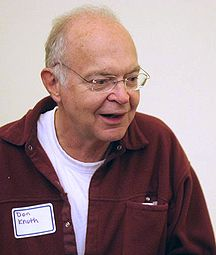
\includegraphics[width=0.25\linewidth]{knuth1}}
        \hfill
    }
    \caption{Подпись к картинке.}\label{fig:latex}
\end{figure}

Формулы в строку без номера добавляются так:
\[
  \lambda_{T_s} = K_x\frac{d{x}}{d{T_s}}, \qquad
  \lambda_{q_s} = K_x\frac{d{x}}{d{q_s}},
\]

\underline{\textbf{Вторая глава}} посвящена исследованию

\underline{\textbf{Третья глава}} посвящена исследованию

Можно сослаться на свои работы в автореферате. Для этого в файле
\verb!Synopsis/setup.tex! необходимо присвоить положительное значение
счётчику \verb!\setcounter{usefootcite}{1}!. В таком случае ссылки на
работы других авторов будут подстрочными.
Изложенные в третьей главе результаты опубликованы в~\cite{vakbib1, vakbib2}.
Использование подстрочных ссылок внутри таблиц может вызывать проблемы.

В \underline{\textbf{четвертой главе}} приведено описание

\FloatBarrier
\pdfbookmark{Заключение}{conclusion}                                  % Закладка pdf
В \underline{\textbf{заключении}} приведены основные результаты работы, которые заключаются в следующем:
%% Согласно ГОСТ Р 7.0.11-2011:
%% 5.3.3 В заключении диссертации излагают итоги выполненного исследования, рекомендации, перспективы дальнейшей разработки темы.
%% 9.2.3 В заключении автореферата диссертации излагают итоги данного исследования, рекомендации и перспективы дальнейшей разработки темы.
\begin{enumerate}
  \item На основе анализа \ldots
  \item Численные исследования показали, что \ldots
  \item Математическое моделирование показало \ldots
  \item Для выполнения поставленных задач был создан \ldots
\end{enumerate}


\pdfbookmark{Литература}{bibliography}                                % Закладка pdf
При использовании пакета \verb!biblatex! список публикаций автора по теме
диссертации формируется в разделе <<\publications>>\ файла
\verb!common/characteristic.tex!  при помощи команды \verb!\nocite!

\ifdefmacro{\microtypesetup}{\microtypesetup{protrusion=false}}{} % не рекомендуется применять пакет микротипографики к автоматически генерируемому списку литературы
\urlstyle{rm}                               % ссылки URL обычным шрифтом
\ifnumequal{\value{bibliosel}}{0}{% Встроенная реализация с загрузкой файла через движок bibtex8
  \renewcommand{\bibname}{\large \bibtitleauthor}
  \nocite{*}
  \insertbiblioauthor           % Подключаем Bib-базы
  %\insertbiblioexternal   % !!! bibtex не умеет работать с несколькими библиографиями !!!
}{% Реализация пакетом biblatex через движок biber
  % Цитирования.
  %  * Порядок перечисления определяет порядок в библиографии (только внутри подраздела, если `\insertbiblioauthorgrouped`).
  %  * Если не соблюдать порядок "как для \printbibliography", нумерация в `\insertbiblioauthor` будет кривой.
  %  * Если цитировать каждый источник отдельной командой --- найти некоторые ошибки будет проще.
  %
  %% authorvak
  \nocite{vakbib1}%
  \nocite{vakbib2}%
  %
  %% authorwos
  \nocite{wosbib1}%
  %
  %% authorscopus
  \nocite{scbib1}%
  %
  %% authorpathent
  \nocite{patbib1}%
  %
  %% authorprogram
  \nocite{progbib1}%
  %
  %% authorconf
  \nocite{confbib1}%
  \nocite{confbib2}%
  %
  %% authorother
  \nocite{bib1}%
  \nocite{bib2}%

  \ifnumgreater{\value{usefootcite}}{0}{
    \begin{refcontext}[labelprefix={}]
      \ifnum \value{bibgrouped}>0
        \insertbiblioauthorgrouped    % Вывод всех работ автора, сгруппированных по источникам
      \else
        \insertbiblioauthor      % Вывод всех работ автора
      \fi
    \end{refcontext}
  }{
  \ifnum \totvalue{citeexternal}>0
    \begin{refcontext}[labelprefix=A]
      \ifnum \value{bibgrouped}>0
        \insertbiblioauthorgrouped    % Вывод всех работ автора, сгруппированных по источникам
      \else
        \insertbiblioauthor      % Вывод всех работ автора
      \fi
    \end{refcontext}
  \else
    \ifnum \value{bibgrouped}>0
      \insertbiblioauthorgrouped    % Вывод всех работ автора, сгруппированных по источникам
    \else
      \insertbiblioauthor      % Вывод всех работ автора
    \fi
  \fi
  %  \insertbiblioauthorimportant  % Вывод наиболее значимых работ автора (определяется в файле characteristic во второй section)
  \begin{refcontext}[labelprefix={}]
      \insertbiblioexternal            % Вывод списка литературы, на которую ссылались в тексте автореферата
  \end{refcontext}
  % Невидимый библиографический список для подсчёта количества внешних публикаций
  % Используется, чтобы убрать приставку "А" у работ автора, если в автореферате нет
  % цитирований внешних источников.
  \printbibliography[heading=nobibheading, section=0, env=countexternal, keyword=biblioexternal, resetnumbers=true]%
  }
}
\ifdefmacro{\microtypesetup}{\microtypesetup{protrusion=true}}{}
\urlstyle{tt}                               % возвращаем установки шрифта ссылок URL
